\section{Interpreter}

O padrão Interpreter define uma representação para 
a gramática de uma linguagem e um interpretador para 
interpretar sentenças dessa linguagem. Apesar da 
descrição generalista, o padrão 
pode ser utilizado para facilitar a resolução de 
problemas que ocorrem com frequência e que podem 
ser definidos através de uma árvore sintática 
abstrata.

Esse padrão pode oferecer riscos quando a gramática 
é complexa. Como para cada regra será necessário 
definir uma nova classe, a hierarquia de classes 
resultante pode tornar-se muito grande e mais 
difícil de controlar. Em contrapartida, é 
fácil modificar ou estender a gramática, já 
que cada regra está encapsulada em uma classe 
diferente. A estrutura do padrão pode ser vista 
no diagrama da imagem \ref{interpreter_struct}.

\begin{figure}[htb]
	\caption{\label{interpreter_struct}Estrutura do Interpreter}
	\begin{center}
	    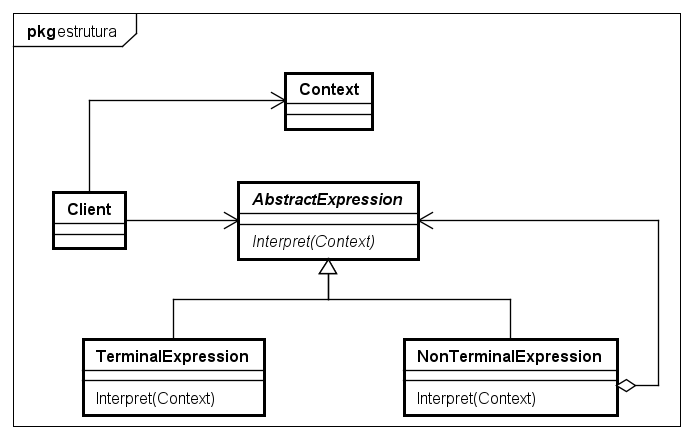
\includegraphics[scale=0.5]{5_padroes-contexto-funcional/5.3_comportamentais/5.3.03_interpreter/Interpreter_struct.png}
	\end{center}
\end{figure}

\subsection*{Exemplo Orientado a Objetos}

Como exemplo, o Interpreter pode ser utilizado para 
interpretar expressões regulares. Cada classe definida 
representa uma regra da gramática, que aceita cadeias de 
caracteres e símbolos de alternação, sequência e 
repetição. No diagrama da figura \ref{interpreter_exemplo}, 
as classes AlternationExpression, RepetitionExpression e 
SequenceExpression representam regras com subexpressões, 
enquanto a classe LiteralExpression representa uma 
regra terminal da gramática. A implementação do exemplo 
pode ser vista no código \ref{oointerpreter}.

\begin{figure}[htb]
	\caption{\label{interpreter_exemplo}Exemplo de Interpreter}
	\begin{center}
	    \includegraphics[scale=0.5]{5_padroes-contexto-funcional/5.3_comportamentais/5.3.03_interpreter/Interpreter_exemplo.png}
	\end{center}
\end{figure}

\begin{lstlisting}[caption={Interpreter Orientação a Objetos},label=oointerpreter]

abstract class RegularExpression {
  def Interpret() : String
}

class LiteralExpression(literal : String) extends RegularExpression {
  def Interpret() : String = literal
}

class SequenceExpression(val expression1 : RegularExpression,
                         val expression2 : RegularExpression)
extends RegularExpression {
  def Interpret() : String = {
    expression1.Interpret() + "&" + expression2.Interpret()
  }
}

class RepetitionExpression(val repetition : RegularExpression)
  extends RegularExpression {

  def Interpret(): String = repetition.Interpret() + "*"
}

class AlternativeExpression(val alternative1 : RegularExpression,
                            val alternative2 : RegularExpression)
extends RegularExpression {

  def Interpret(): String = {
    alternative1.Interpret() + " | " + alternative2.Interpret()
  }
}
    
\end{lstlisting}

\subsection*{Contexto Funcional}

\begin{comment}
O próprio GoF cita pattern matching como um exemplo de 
aplicação do padrão Interpreter. Apesar de não ser um 
conceito necessariamente funcional, pattern matching costuma 
ser nativamente implementado por linguagens como Haskell e 
Scala. As linguagens funcionais também costumam implementar 
de forma mais simples tipos algébricos, que são definidos 
quase identicamente às gramáticas usadas para definir 
linguagens. Dessa forma, o que antes necessitaria de diversas 
classes e interfaces para uma hierarquia que não poderia 
ser muito complexa, pode ser traduzido como uma função 
que aproveita o pattern matching naturalmente para decidir 
e interpretar um valor definido através de um tipo abstrato.
\end{comment}

\begin{lstlisting}[caption={Interpreter Funcional},label=fpinterpreter]
    

    
\end{lstlisting}